\chapter{Methodology}\label{ch:methodology}

This section outlines the complete modeling framework used to determine the equilibrium and
stability limits of hydrogen exsolution at the magma-atmosphere boundary of sub-Neptune
exoplanets, called the core--envelope boundary in \cite{gilmore2026}. The implementation is
performed using \Atm{} \cite{bower2025}, an open-source Python library designed to resolve
coupled chemical equilibrium and mass-balance constraints in gas-melt environments. In the
following sections, we outline the conceptual basis, numerical approach, chemical system,
and software validation.

\section{Formulation and Numerical Solution}

\subsection{Solver Architecture}

Users define the gaseous species, from which the software generates an independent reaction
basis using Gaussian elimination (Leal et al.\ 2016 \cite{leal2016}). At the interface, the
solver determines chemical equilibrium among gas species and any specified dissolved species
within the melt, subject to elemental mass conservation. The solver determines the
equilibrium state by minimizing the total Gibbs free energy using the optimistix framework,
with
\begin{equation}
G = \sum_i n_i \mu_i(T,P),
\label{eq:gibbs}
\end{equation}
where $n_i$ is the number of moles and $\mu_i$ is the chemical potential of species $i$,
which includes EOS corrections and melt interactions. \Atm{} employs the extended law of mass
action (xLMA; Leal et al.\ 2016 \cite{leal2016}) to build a closed nonlinear system that
integrates equilibrium chemistry with elemental mass balance, structured as a root-finding
problem, and leverages JAX for high-performance computations (Bradbury et al.\ 2018
\cite{jax2018}). The nonlinear system is resolved using robust Newton--type root--finders
augmented with line--search and trust--region safeguards.

For this work we extended the phase-equilibrium module of \Atm{}. A binary mixing model now
supplies the nonideal activities of two condensed components, here MgSiO$_3$ and H$_2$. The
same Gibbs energy yields the homogeneous activities, the coexisting compositions, the local
stability and the equilibrium (convex-envelope) free energy, so that all quantities in this
work follow from one function.

\subsection{Phase Equilibrium and Local Stability}

For a binary mixture with molar Gibbs energy of mixing $g_{\rm mix}(x)$, two phases $\alpha$
and $\beta$ coexist when both component chemical potentials are equal,
\begin{equation}
\mu_{\rm sil}^{\alpha} = \mu_{\rm sil}^{\beta},\qquad
\mu_{\rm H_2}^{\alpha} = \mu_{\rm H_2}^{\beta},
\label{eq:coexistence}
\end{equation}
which is the common-tangent construction. The locus of coexisting compositions as a function
of temperature is the \textbf{binodal}. A homogeneous mixture is locally stable as long as
\begin{equation}
\frac{\partial^2 g_{\rm mix}}{\partial x^2} > 0,
\label{eq:stability}
\end{equation}
and the locus where this curvature vanishes is the \textbf{spinodal}. Between the binodal and
the spinodal a homogeneous mixture is metastable: it is stable against small composition
fluctuations, but a nucleus of the other phase that exceeds a critical size lowers the free
energy \cite{debenedetti1996}. Inside the spinodal it decomposes spontaneously
\cite{cahn1961}. Both conditions are evaluated with bracketed root finding on the two stable
branches, which excludes the trivial equal-composition solution, and with implicit
derivatives for use inside the \Atm{} solver.

\section{Hydrogen--Silicate Mixing Model}\label{sec:mixing_model}

Gilmore \& Stixrude \cite{gilmore2026} describe their phase-coexistence and homogeneous
DFT-MD simulations with an asymmetric regular solution model. We write their equation~8 as
\begin{equation}
\begin{split}
g_{\rm mix} ={}& W(x)\left(1-\frac{T}{\tau}+\frac{P}{\pi}\right)\\
 &+ RT\left[x\ln x + (1-x)\ln(1-x)\right],
\end{split}
\label{eq:gs26}
\end{equation}
with the excess enthalpy at zero pressure
\begin{equation}
W(x) = x(1-x)\left[A(1-x)+Bx\right],
\label{eq:w}
\end{equation}
excess entropy $W/\tau$ and excess volume $W/\pi$. The published parameters are
$A = 75$\,kJ\,mol$^{-1}$, $B = 424$\,kJ\,mol$^{-1}$, $\tau = 4{,}400$\,K and
$\pi = -35$\,GPa. The composition variable is the molar fraction of the H$_2$ component on an
oxide basis,
\begin{equation}
\begin{split}
x &= \frac{N_{\rm H_2}}{N_{\rm H_2}+N_{\rm MgO}+N_{\rm SiO_2}}\\
  &= \frac{N_{\rm H}/2}{N_{\rm H}/2 + 2(N_{\rm Mg}+N_{\rm Si}+N_{\rm O})/5}.
\end{split}
\label{eq:x}
\end{equation}
The paper does not state which component carries $A$ and which carries $B$. The critical
temperature is the same for both choices, but the shape of the miscibility gap is not.
Assigning $B$ to the H$_2$-rich side (Eq.~\ref{eq:w}) reproduces the published curves of
their Figure~2 and their statement that the hydrogen-poor phase holds more hydrogen than the
hydrogen-rich phase holds silicate (Section~\ref{sec:verification}).

\paragraph{Composition basis.} \Atm{} uses native formula units, with the H$_2$ fraction
$y = n_{\rm H_2}/(n_{\rm H_2}+n_{\rm MgSiO_3})$. One MgSiO$_3$ unit contains two oxide units,
so
\begin{equation}
x = \frac{y}{2-y}, \qquad
G = \left(2\,n_{\rm MgSiO_3} + n_{\rm H_2}\right) g_{\rm mix}(x).
\label{eq:basis}
\end{equation}
The second relation keeps the free energy extensive; the native chemical potentials are
$\mu_{\rm MgSiO_3} = 2\mu_{\rm oxide}$ and $\mu_{\rm H_2}$. Converting only the endpoint
compositions is not sufficient, because the native curvature, activities and phase amounts
all depend on the factor $2-y$. We implemented this conversion as a static multiplicity of
the silicate component, available through the constructor
\texttt{hydrogen\_silicate\_gilmore26} of the class \texttt{SubregularSolution}.

\paragraph{Controls.} As controls we retain the historical 2025 parameterization of Rogers,
Young \& Schlichting \cite{rogers2025} on its own formula-unit basis, and a deliberately
incorrect import of the 2026 parameters without the basis conversion. The latter is a
diagnostic, never a recommended model.

\section{Delayed-Exsolution Limit}\label{sec:delayed}

We follow a closed, initially homogeneous parcel that cools at fixed pressure. Its local
hydrogen mass fraction $w$ fixes $y$ and hence $x$. On cooling it first enters the
miscibility gap at the binodal temperature $T_b(w,P)$ and later becomes locally unstable at
the spinodal temperature $T_{\rm sp}(w,P)$. Because Eq.~(\ref{eq:gs26}) is linear in $T$,
the spinodal temperature follows analytically from Eq.~(\ref{eq:stability}):
\begin{equation}
T_{\rm sp} = \frac{-W''(x)\,(1+P/\pi)}{R/[x(1-x)] - W''(x)/\tau}.
\label{eq:tsp}
\end{equation}
We compare two limiting histories. In the \textbf{equilibrium limit} the parcel separates as
soon as it crosses $T_b$. In the \textbf{delayed limit} nucleation is suppressed until
$T_{\rm sp}$, after which the parcel equilibrates rapidly. We report the metastable interval
\begin{equation}
\Delta T_{\rm ms} = T_b - T_{\rm sp},
\label{eq:interval}
\end{equation}
and the fraction of all hydrogen that the equilibrium limit already places in the H-rich
phase at $T_{\rm sp}$,
\begin{equation}
f_{\rm H} = \frac{\phi\, y_{\rm rich}}{y_0}, \qquad
\phi = \frac{y_0-y_{\rm poor}}{y_{\rm rich}-y_{\rm poor}},
\label{eq:fh}
\end{equation}
where $\phi$ is the native mole fraction of the H-rich phase from the lever rule. The quantity
$f_{\rm H}$ is the largest inventory that the delayed limit can withhold from separation. It is
a bound between two assumptions, not a computed release rate: both histories conserve all
hydrogen, and the delayed parcel still holds its hydrogen dissolved in the silicate.

\section{Model Configurations and Parameter Space}

The results presented in the Results are derived from sweeps over four parameters. When
varying a specific parameter, the other three are held at their baseline values unless
otherwise noted.
\begin{enumerate}
\item \textbf{Local Hydrogen Mass Fraction (0.1\% -- 20\%):} This range spans parcels from
silicate-rich melt to hydrogen-rich fluid at the magma-atmosphere boundary.\\
\textit{Baseline:} $w = 3$\,wt\%, a composition that crosses both the binodal and the
spinodal above 2,000\,K.
\item \textbf{Pressure (2 -- 10\,GPa):} This range covers most of the magma-atmosphere
boundary pressures of the sub-Neptune models compiled in \cite{gilmore2026}.\\
\textit{Baseline:} $P = 2$\,GPa, the pressure of the best-sampled simulations.
\item \textbf{Temperature (2,000\,K -- 4,000\,K):} This window covers the fluid regime of the
simulations. We report spinodals below 2,000\,K separately and test stopping temperatures of
2,500 and 3,000\,K, because neither is a computed melting boundary.
\item \textbf{Mixing Model:} the published 2026 fit (baseline), the historical 2025 fit and
the incorrect-basis control, and the recalibrated model classes of
Section~\ref{sec:recalibration}.
\end{enumerate}
In total the onset grid contains \nOnsetRows{} rows and the cooling paths \nCoolingRows{}
states. A further \nStressRows{} deterministic stress cases change $A$, $B$, $\tau$ and
$|\pi|$ by $\pm10\%$, individually and in combination. These stress cases are not calibrated
uncertainties; Section~\ref{sec:recalibration} replaces them with data-driven posteriors.

\section{Source-Data Audit and Recalibration}\label{sec:recalibration}

\subsection{Source Data}

The source simulations are public \cite{gilmore2026data}. Extended Data (ED) Table~1 lists
14 phase-coexistence runs: four that kept two phases, with the composition of each phase, and
ten that became one homogeneous phase, with their bulk composition. The quoted composition
uncertainty is $\pm0.05$ in $x$. ED Table~2 lists homogeneous simulations at 5\,GPa and
4,000\,K: three mixtures and the two endmembers, with enthalpy, entropy and volume per atom.
We reconstruct excess properties per mole of mixing units (Eq.~\ref{eq:x}) and remove the
ideal mixing entropy from the total entropy. The endmember errors are shared between the
three mixtures, so we propagate a full covariance matrix. The endmembers were simulated at
5.00\,GPa and the mixtures at 5.06--5.08\,GPa; we add the corresponding enthalpy and volume
shifts as a fully correlated systematic error. Finally, we digitized the published
Figure~2a, which shows the same coexistence runs, from the CC-BY figure file.

\subsection{Likelihood and Model Classes}

We compare models with the data through three terms,
\begin{equation}
\chi^2 = \chi^2_{\rm phase} + \chi^2_{\rm comp} + \chi^2_{\rm hom}.
\label{eq:chi2}
\end{equation}
The first term uses the most robust information in the source: whether each of the 14 runs
kept one or two phases. A model that misplaces a run pays
$[(T_{\rm run}-T_b)/\sigma_T]^2$, with $T_b$ the model binodal temperature at the run's bulk
composition and $\sigma_T^2 = (50\,{\rm K})^2 + (100\,{\rm K\,GPa^{-1}}\,\sigma_P)^2$, which
adds the quoted pressure error. The second term compares the eight coexisting compositions,
with the quoted $\pm0.05$ treated as a Gaussian standard deviation. The third term compares
the nine homogeneous excess properties with their covariance.

We fit four smooth model classes with constant excess enthalpy, entropy and volume, so that
their spinodals follow in closed form. They are written as Redlich--Kister series
\cite{redlich1948},
\begin{equation}
G_{\rm ex} = \sum_k \left(h_k - T s_k + P v_k\right) x(1-x)(1-2x)^k,
\label{eq:rk}
\end{equation}
summarized in Table~\ref{tab:classes}. Class M1 is the published form. M2 frees the shapes
of the excess entropy and volume. M3 and M4 add one and two higher composition terms that
share the published temperature and pressure scaling.

\begin{table}[t]
\thesiscaption{Model classes used in the recalibration.}{All classes have constant excess
enthalpy, entropy and volume coefficients. The last column counts free parameters.}
\label{tab:classes}
\small\centering
\begin{tabular}{@{}llc@{}}
\toprule
Class & Excess Gibbs energy & $n$\\
\midrule
M1 & published form, Eq.~(\ref{eq:gs26}) & 4\\
M2 & subregular $H$, $S$ and $V$, independent & 6\\
M3 & RK order 2, published $T,P$ scaling & 5\\
M4 & RK order 3, published $T,P$ scaling & 6\\
\bottomrule
\end{tabular}
\end{table}

Priors are uniform within broad stated bounds; we sample $1/\tau$ and $1/\pi$ rather than
$\tau$ and $\pi$. We draw posterior samples with an adaptive Metropolis algorithm
\cite{haario2001}: eight chains of 12,000 steps, of which the first 3,000 adapt the proposal
and are discarded. We check convergence with the split-chain $\hat R$ statistic
\cite{gelman2013}. Besides the full data set we fit five variants of class M1: with the
Figure~2a compositions, with $\sigma_x = 0.15$ for the two runs closest to $T_C$, without
the excess volumes, and with only the phase states plus either the compositions or the
homogeneous data. For every retained sample we recompute $T_b$, $T_{\rm sp}$,
$\Delta T_{\rm ms}$, $f_{\rm H}$ and $T_C$ at the baseline.

\subsection{Identifiability Test}

To test whether coexistence data can identify the spinodal at all, we add a nonnegative
perturbation that lives only inside the miscibility gap,
\begin{equation}
\delta g = 64\,\lambda B_{\rm gap}\, u^3(1-u)^3,\quad
u = \frac{x-x_{\rm poor}}{x_{\rm rich}-x_{\rm poor}},
\label{eq:bump}
\end{equation}
for $x_{\rm poor}<x<x_{\rm rich}$ and zero elsewhere. Here $B_{\rm gap}$ is the height of the
published free energy above its common tangent at the middle of the gap. The perturbation and
its first two derivatives vanish at the binodal, so all coexisting compositions, all
equilibrium free energies and all homogeneous states outside the gap stay exactly the same.
The amplitudes $\lambda = 0$ to 8 are a counterexample to uniqueness, not a material model.

\section{Verification of Thermodynamic Consistency}\label{sec:verification}

We verified the implementation in three independent ways. First, our implementation
reproduces the published model. Its critical temperatures are \pubTcTwo{}\,K at 2\,GPa and
\pubTcTen{}\,K at 10\,GPa, matching the published 3,500 and 2,600\,K, and our binodals follow
the digitized curves of the published Figure~2a with an RMS residual of at most \digRms{}\,K
(Figure~\ref{fig:verification}a). The largest single deviation, \digMax{}\,K, is about three
pixels of the printed line.

Second, a separate scalar implementation, written without any code from \Atm{}, agrees with
the \Atm{} binodal and spinodal temperatures to within \indepMaxDiff{}\,K over the grid
(Figure~\ref{fig:verification}b). The exception is the binodal within 0.02 of $x_C$, where the
flat crest makes the binodal temperature ill-conditioned and the two codes differ by up to
\indepMaxDiffCrit{}\,K. It locates spinodal compositions as the real roots of a
polynomial and binodals by nested bracketed root finding, so its errors are independent of
the \Atm{} solver.

Third, the \Atm{} test suite passed \nTests{} tests, including the extensive-energy
derivative test of the basis conversion (Eq.~\ref{eq:basis}), Gibbs--Duhem consistency and
spinodal temperatures against independent roots. The study itself checks conservation of
each native component in \nNativeSolves{} native equilibrium solves and compares 30 spinodal
temperatures with independent SciPy roots. The largest elemental and lever-rule errors are
$2.2\times10^{-16}$.

\begin{figure*}[t]
\centering
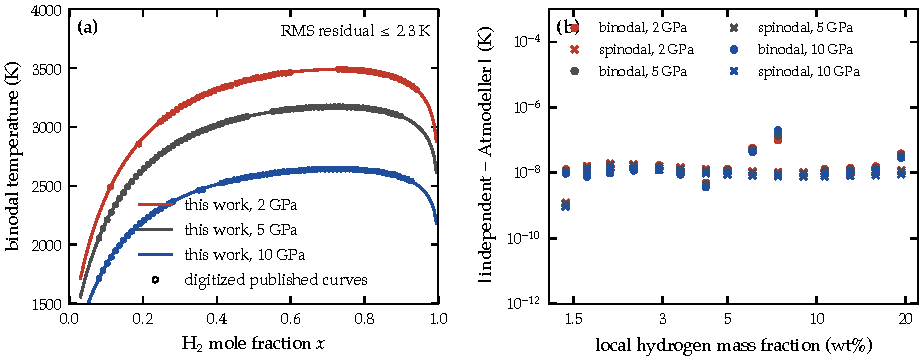
\includegraphics[width=\textwidth]{fig2_1_verification}
\thesiscaption{Internal consistency check of \Atm{}.}{(a) Binodal temperatures of our
implementation of Eq.~(\ref{eq:gs26}) (lines) and the curves digitized from Figure~2a of
\cite{gilmore2026} (circles) at 2, 5 and 10\,GPa. (b) Absolute difference between a separate
scalar implementation and \Atm{} for the binodal (circles) and spinodal (crosses)
temperatures across the onset grid. The two codes share no solver code.}
\label{fig:verification}
\end{figure*}

\section{Data Processing, Model Limitations and Assumptions}

\subsection{Data Processing}

Model outputs were exported as CSV and JSON files with SHA-256 hashes of every artifact and
analysis script. Data reduction was performed using pandas, and visualizations were generated
using matplotlib. Key diagnostics reported in the Results include the binodal and spinodal
temperatures, the metastable interval $\Delta T_{\rm ms}$, the withheld hydrogen fraction
$f_{\rm H}$ and the critical temperature $T_C$.

\subsection{Model Limitations and Assumptions}

The current framework operates under several constraints. First, the mixture is a binary
H$_2$--MgSiO$_3$ system; helium, iron and other volatiles are absent, and the source
simulations used pure MgSiO$_3$. Second, all model classes have constant excess enthalpy,
entropy and volume, so the free energy is linear in temperature and pressure. Third, the
local mass fractions describe a closed parcel; we do not model transport between the
interior and the envelope, convection or settling. Finally, the approach treats nucleation
only as two limiting cases, neglecting nucleation rates, interfacial energies,
diffusion-limited growth and spatial gradients within the reservoirs.
